\documentclass[aspectratio=169]{beamer}
\usepackage{will_handley_beamer}
\usepackage{title_page}

% Commands
% --------
% - \arxiv{arxiv number}
% - \arxiv{<number>}            arxiv.org/abs/<number>
% - \oldarxiv{<arxiv number>}   arxiv.org/<number>
% - \doi{<doi>}                 doi.org/<doi>
% - \xkcd{<number>}             xkcd.com/<number>
% - \email{<email>}             <<email>>
% - \tthref{<website>}          <website>
% - \av[dist]{<quantity>}       <quantity>_{dist}
% - \student{<name>}{<detail>}{<photo>}

% Talk details
% ------------
\title{Cosmic Tensions}
\subtitle{A High Energy Physicist's Primer}
\date{31\textsuperscript{st} January 2025}

\begin{document}

\begin{frame}
    \titlepage
\end{frame}

\begin{frame}
    \frametitle{Introduction: Precision Cosmology and its Discontents}
    \vspace{-0.1cm}
    \begin{columns}
        \column{0.5\textwidth}
        \begin{itemize}
            \item Have well-and-truly entered an era of precision cosmology.
            \item Multiple independent observations allow us to constrain the parameters of our cosmological model.
            \item The Standard Model of Cosmology ($\Lambda$CDM) successfully explains a wide range of observations.
            \item However, increasing precision has revealed inconsistencies, or tensions, between different measurements.
            \item Are these tensions cracks in $\Lambda$CDM, hints of new physics, or simply measurement systematics?
        \end{itemize}
        \column{0.5\textwidth}
        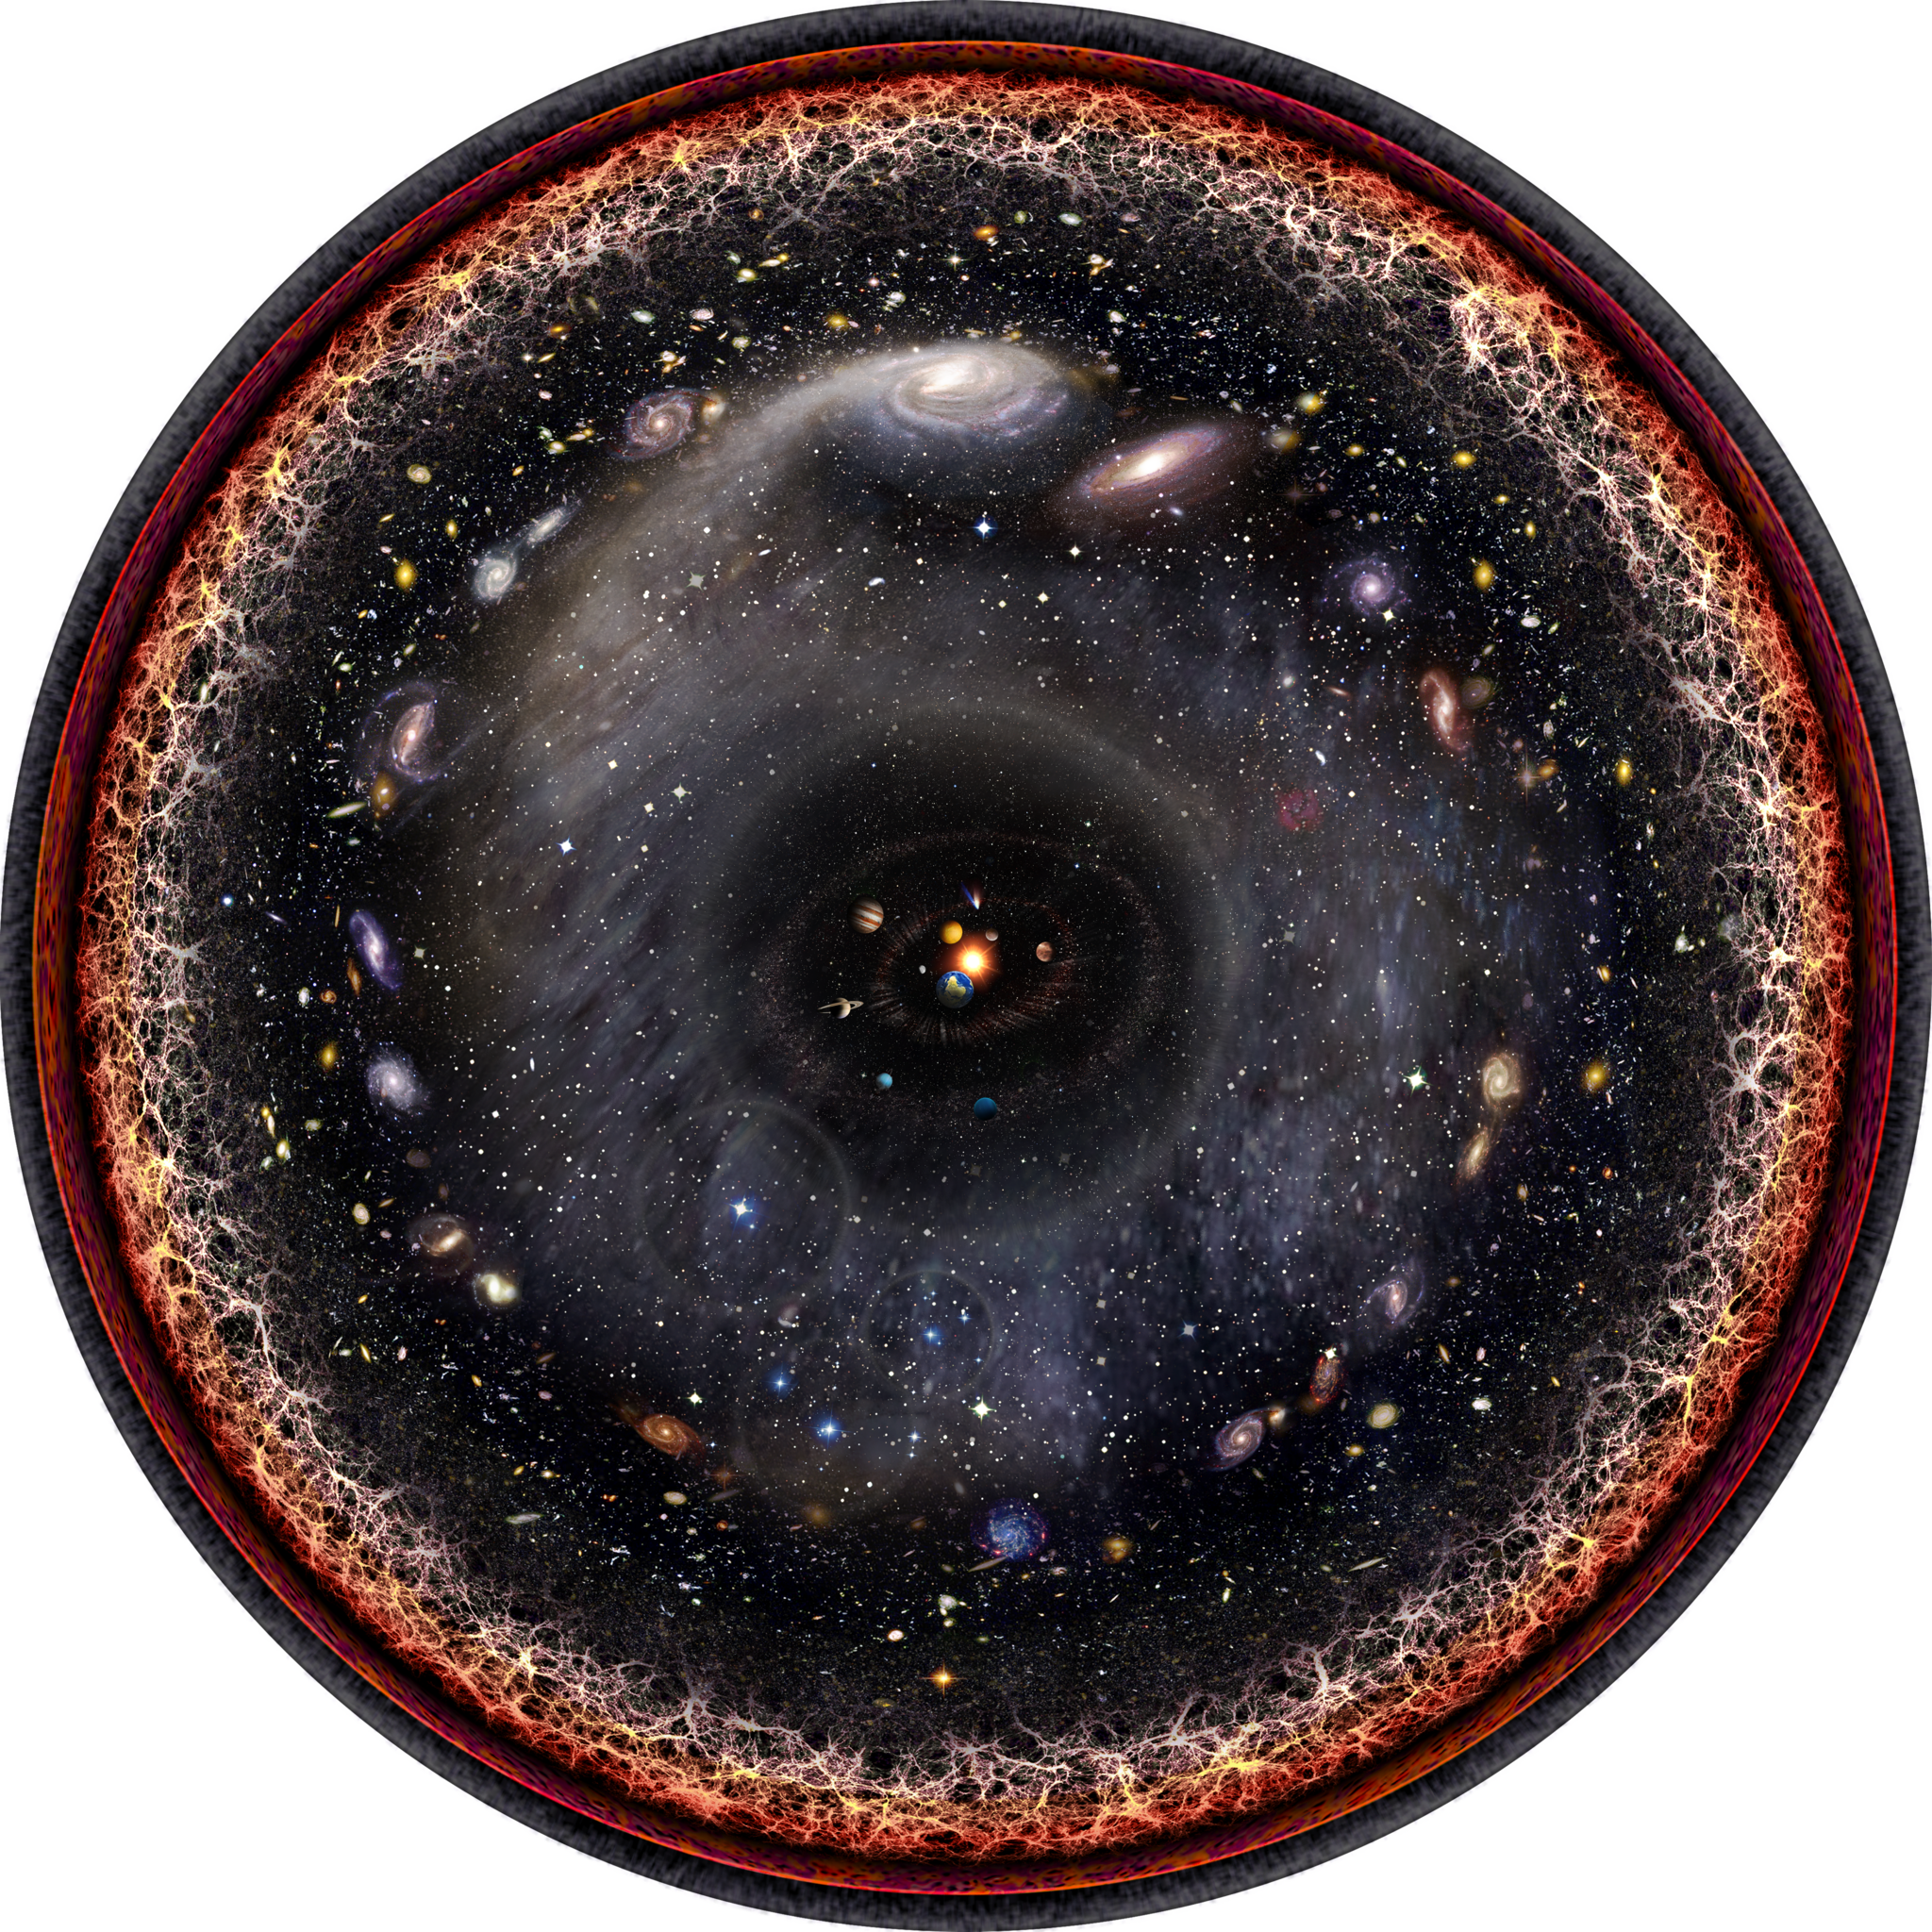
\includegraphics[width=\textwidth]{figures/cosmos.png}
    \end{columns}
\end{frame}

\begin{frame}
    \frametitle{Measuring the Universe}
    \begin{columns}
        \column{0.53\textwidth}
        \begin{itemize}
            \item How do you know how far away anything is?
                \begin{itemize}
                    \item<2-> Beyond our arms reach (where stereopsis fails), we rely on parallax between objects picked up by slight head motion.
                \end{itemize}
            \item<3-> Parallax is the archetypal cosmological \textbf{geometric} measurement\ldots
            \item<4-> \ldots but it only gets you so far.
            \item<5-> To go beyond parallax you need:
                \begin{itemize}
                    \item<5-> a standardisable object that exists next to your geometric measurements\ldots
                    \item<5-> \ldots or some other way to measure distance.
                \end{itemize}
        \end{itemize}
        \column{0.47\textwidth}
        \includegraphics<3>[width=\textwidth]{figures/parallax_geom.jpg}% 
        \includegraphics<4->[width=\textwidth]{figures/parallax.png}
    \end{columns}
\end{frame}


\begin{frame}
    \frametitle{Standard Candles}
    \framesubtitle{Supernovae}
    \begin{columns}
        \column{0.5\textwidth}
        \begin{itemize}
            \item <+SH0ES+>
            \item <+CCHP+>
            \item <+Type Ia+>
            \item <+Cepheids+>
            \item <+TRGB stars+>
            \item <+JAGB stars+>
        \end{itemize}
        \column{0.5\textwidth}
        \includegraphics<1>[width=\textwidth]{figures/candles.jpg}%
        \only<2>{
            \begin{overpic}[width=\textwidth]{figures/Dist_Ladd_distance_ladder_R22.pdf}
                \put(0,65){\includegraphics[width=0.3\textwidth]{figures/type_ia.jpg}}
                \put(60,0){\includegraphics[width=0.4\textwidth]{figures/cepheid.jpg}}
                \put(70,25){\includegraphics[width=0.3\textwidth]{figures/cepheid_curve.jpg}}
            \end{overpic}
        }
    \end{columns}
\end{frame}

\begin{frame}
    \frametitle{Standard Rulers}
    \begin{columns}
        \column{0.55\textwidth}
        \begin{itemize}
            \item <+CMB+>
            \item <+BAO+>
            \item <+Strong lensing+>
            \item <+Weak lensing+>
        \end{itemize}
        \column{0.45\textwidth}
        \includegraphics[width=\textwidth]{figures/rulers.jpg}
    \end{columns}
\end{frame}

\begin{frame}
    \frametitle{Standard Rulers}
    \framesubtitle{The cosmic microwave background}
    \begin{columns}
        \column{0.55\textwidth}
        \begin{itemize}
            \item <+CMB+>
        \end{itemize}
        \column{0.45\textwidth}
        \includegraphics[width=\textwidth]{figures/cmb.png}
        \includegraphics[width=\textwidth]{figures/cmb_power_spectrum.jpg}%
    \end{columns}
\end{frame}

\begin{frame}
    \frametitle{Standard Rulers}
    \framesubtitle{Baryon Acoustic Oscillations}
    \begin{columns}
        \column{0.55\textwidth}
        \begin{itemize}
            \item <+Explanation+>
            \item <+SDSS+>
            \item <+DESI+>
        \end{itemize}
        \column{0.45\textwidth}
        \includegraphics[width=\textwidth]{figures/desi_galaxies.png}
        \includegraphics[width=\textwidth]{figures/desi_bao.jpg}%
    \end{columns}
\end{frame}

\begin{frame}
    \frametitle{Standard Rulers}
    \framesubtitle{Strong Lensing}
    \begin{columns}
        \column{0.55\textwidth}
        \begin{itemize}
            \item <+Explanation+>
            \item <+Planck+>
        \end{itemize}
        \column{0.45\textwidth}
        \includegraphics[width=\textwidth]{figures/time_delay.jpg}
        \includegraphics[width=\textwidth]{figures/time_delay_curve.png}%
    \end{columns}
\end{frame}

\begin{frame}
    \frametitle{Standard Rulers}
    \framesubtitle{Weak Lensing}
    \begin{columns}
        \column{0.55\textwidth}
        \begin{itemize}
            \item <+DES+>
            \item <+KiDS+>
            \item <+HSC+>
        \end{itemize}
        \column{0.45\textwidth}
        \includegraphics[width=\textwidth]{figures/weak_lensing.png}
    \end{columns}
\end{frame}

\begin{frame}
    \frametitle{Standard Sirens}
    \begin{columns}
        \column{0.5\textwidth}
        \begin{itemize}
            \item <+Bright sirens+>
            \item <+Dark sirens+>
            \item <+Spectral sirens+>
        \end{itemize}
        
        \column{0.5\textwidth}
        \includegraphics[height=0.33\textwidth]{figures/gw.jpg}%
        \includegraphics[height=0.33\textwidth]{figures/gw_local.jpg}
        \includegraphics[width=\textwidth]{figures/posterior_O3_dr9beta_170817.png} % 2111.06445
        
    \end{columns}
\end{frame}

\begin{frame}
    \frametitle{Standard Clocks}
    \begin{columns}
        \column{0.5\textwidth}
        \begin{itemize}
            \item <+Cosmic Chronometers+>
            \item <+Pulsar timing arrays+>
        \end{itemize}
        \column{0.5\textwidth}
        %\includegraphics[width=\textwidth]{figures/clocks.jpg}
        \includegraphics[width=\textwidth]{figures/timers.jpg}
    \end{columns}
\end{frame}
 
\begin{frame}
    \frametitle{The Hubble tension}
    \begin{columns}
        \column{0.5\textwidth}
        \begin{itemize}
            \item CMB: $H_0=67.4\pm0.5$ km/s/Mpc.
            \item S$H_0$ES: $H_0=73.2\pm1.3$ km/s/Mpc.
            \item Exciting if not measurement error
                \begin{itemize}
                    \item People trust the CMB measurement, but perhaps not $\Lambda$CDM model
                    \item Measurements of $H_0$ from supernovae notoriously challenging
                \end{itemize}
            \item As of 2024 Hubble three ways (Cepheids, TRGB, JAGB)
                \begin{description}
                    \item [Friedmann] $H_0 = (72.0, 69.8, 67.96)\pm1.8$ 
                    \item [Riess] $H_0 = (73.4, 72.1, 72.2)\pm2.2$ 
                \end{description}                                      
                \hfill\arxiv{2408.06153}\arxiv{2408.11770}
        \end{itemize}
        \column{0.5\textwidth}
        \includegraphics<1>[width=\textwidth]{figures/H0_1.jpg}%
        \includegraphics<2>[width=\textwidth]{figures/H0_2.jpg}%
        \includegraphics<3>[width=\textwidth]{figures/H0_3.png}%
        \includegraphics<4>[width=\textwidth]{figures/H0_4.png}%
        \only<5>{
            \begin{overpic}[height=0.9\textheight]{figures/hH0whisker_Chapter2_SameRowColor4_SN_P15.pdf}
                \put(18,4){\tiny\arxiv{2103.01183}}
            \end{overpic}
        }
    \end{columns}
\end{frame}

\begin{frame}
    \frametitle{The $S_8$ tension}
    \framesubtitle{aka $\sigma_8$/weak lensing tension}
    \begin{columns}
        \column{0.52\textwidth}
        \begin{itemize}
            \item $S_8$ quantifies the amplitude of matter fluctuations on large scales.
            \item $S_8=\sqrt{\sigma_8(\Omega_m/0.3)^{0.5}}$.
        \end{itemize}
        \column{0.48\textwidth}
        \includegraphics<1>[width=\textwidth]{figures/K+Dcontour_sig8om.pdf}%
        \includegraphics<2>[width=\textwidth]{figures/K+Dcontour.pdf}%
        \only<3>{%
        \begin{overpic}[width=\textwidth]{figures/s8_tension.pdf}
            \put(0,0){\arxiv{2402.08458}}
        \end{overpic}}
    \end{columns}
    \arxiv{2305.17173}
\end{frame}


\begin{frame}
    \frametitle{Other Tensions and Anomalies}
    \begin{columns}
        \column{0.5\textwidth}
        \begin{itemize}
            \item $A_{\rm lens}$ anomaly \arxiv{1807.06209 }
            \item Non-zero curvature \arxiv{1902.04029}
            \item CMB anisotropic anomalies \arxiv{1510.07929}
            \item BBN anomalies \arxiv{1912.01132}
        \end{itemize}
        \column{0.5\textwidth}
        \begin{overpic}[width=\textwidth]{figures/omegak_H0.pdf} 
            \put(0,0){\tiny\arxiv{1908.09139}}
        \end{overpic}
        \includegraphics[width=\textwidth]{figures/lithium.pdf}
    \end{columns}
\end{frame}

\begin{frame}
    \frametitle{Cosmology in 2024}
    \begin{columns}
        \column{0.5\textwidth}
        \begin{itemize}
            \item 2024 was a big year for cosmology:
                \begin{description}
                    \item[Jan] DESY5 SNe \arxiv{2401.02929}
                    \item[Feb] eROSITA \arxiv{2402.08458}
                    \item[Mar] DESI \arxiv{2404.03002}
                \end{description}
        \end{itemize}
        \column{0.5\textwidth}
        \includegraphics[width=\textwidth]{figures/HD_5yr_KeyPaper.pdf}
        \includegraphics[height=0.42\textwidth]{figures/LCDM_paper.pdf}%
        \includegraphics[height=0.42\textwidth]{figures/w0wa_paper_wZoom.pdf}
    \end{columns}
\end{frame}

\begin{frame}
    \frametitle{eROSITA}
    \begin{columns}
        \column{0.5\textwidth}
        \begin{itemize}
            \item <+Paper+> \arxiv{2402.08458}
        \end{itemize}
        \column{0.5\textwidth}
        \includegraphics[width=\textwidth]{figures/eROSITA.pdf}
    \end{columns}
\end{frame}

\begin{frame}
    \frametitle{DESI}
    \begin{columns}
        \column{0.5\textwidth}
        \begin{itemize}
            \item <+Cosmology+> \arxiv{2404.03002}
            \item <+Data+> \arxiv{2404.03000}
        \end{itemize}<++>
        \column{0.5\textwidth}
        \includegraphics[width=\textwidth]{figures/w0wa_DESI-Planck-SN-95lim.pdf}
    \end{columns}
\end{frame}

\begin{frame}
    \frametitle{What to watch out for}
    \begin{columns}
        \column{0.33\textwidth}
        \begin{itemize}
            \item In 2025
                \begin{itemize}
                    \item DESI: BAO
                    \item DES/Euclid: Weak lensing
                    \item eROSITA: X-ray clusters
                    \item ACT: CMB
                    \item LIGO(LVK): GWs
                \end{itemize}
            \item Next 5 years
                \begin{itemize}
                    \item Simons Observatory: CMB
                    \item Rubin: Strong lensing
                    \item Roman: [Hubble 3.0]
                    \item IPTA: Pulsar timing arrays
                \end{itemize}
            \item Next 10-20 years
                \begin{itemize}
                    \item LISA/Einstein: GWs
                    \item SKA: FRBs
                    \item LiteBird: CMB
                    \item ATHENA: X-ray clusters
                \end{itemize}
        \end{itemize}
        \column{0.67\textwidth}
        \includegraphics[height=0.145\textwidth]{figures/telescopes/jwst.png}%
        \includegraphics[height=0.145\textwidth]{figures/telescopes/roman.jpg}%
        \includegraphics[height=0.145\textwidth]{figures/telescopes/euclid.jpeg}%
        \includegraphics[height=0.145\textwidth]{figures/telescopes/athena.jpg}%
        \includegraphics[height=0.145\textwidth]{figures/telescopes/lisa.jpg}%
        \includegraphics[height=0.145\textwidth]{figures/telescopes/e-ASTROGAM.pdf}%
        \vspace{-1pt}
        \includegraphics[height=0.15183\textwidth]{figures/telescopes/desi.jpg}%
        \includegraphics[height=0.15183\textwidth]{figures/telescopes/eelt.jpg}%
        \includegraphics[height=0.15183\textwidth]{figures/telescopes/ska.jpg}%
        \includegraphics[height=0.15183\textwidth]{figures/telescopes/SO.jpg}%
        \vspace{-1pt}
        \includegraphics[height=0.18428\textwidth]{figures/telescopes/ligo.jpg}%
        \includegraphics[height=0.18428\textwidth]{figures/telescopes/km3n.jpg}%
        \includegraphics[height=0.18428\textwidth]{figures/telescopes/icecube.jpg}%
        \includegraphics[height=0.18428\textwidth]{figures/telescopes/CTA.jpg}%
    \end{columns}
\end{frame}

\end{document}
